\documentclass{article}

% Language setting
% Replace `english' with e.g. `spanish' to change the document language
\usepackage[english]{babel}

% Set page size and margins
% Replace `letterpaper' with `a4paper' for UK/EU standard size
\usepackage[letterpaper,top=2cm,bottom=2cm,left=3cm,right=3cm,marginparwidth=1.75cm]{geometry}

% Useful packages
\usepackage{amsmath}
\usepackage{graphicx}
\usepackage[colorlinks=true, allcolors=blue]{hyperref}
\usepackage{caption}
\captionsetup{justification=centering}

\title{Airfoil Analysis}
\author{Ryan Howell}

\begin{document}
\maketitle

%\begin{abstract}

%\end{abstract}

\section{Introduction}

Through reading the textbook and Xfoil.jl documentation as a part of this assignment I learned about the panel method. By experimenting with Xfoil.jl functions I observed the aerodynamic effects of airfoils. In this report I will discuss some key takeaways from the reading and will explore the effects of manipulating the airfoil shape and environmental conditions using the panel method. These results will be verified through comparison with published experimental, CFD and Xfoil data.

\section{Background Readings}
The textbook covers the basic aerodynamics of airfoils, the NACA airfoil, and the panel method's underlying approach and assumptions. These are central to understanding how the Xfoil functions work and how to interpret its results. This section highlights key takeaways from the readings.
\subsection{Airfoils}
The forces acting on a airfoil include a lift force perpendicular to the free stream velocity and a drag force acting in line with the free stream velocity. The chord of the airfoil, drawn directly between the leading and trailing edges, serves as a reference point. The angle of attack, the angle between the chord line and the free-stream flow, along with other properties such as Reynolds number and airfoil shape, affect the behavior and performance of the airfoil.
\subsection{NACA Standardization}
The NACA airfoil consists of numbers relating to the maximum camber, distance of the maximum camber from the leading edge, and the maximum thickness of the airfoil. 
The first number relates to the maximum camber, referring to the maximum distance between the chord and the camber line. The camber line is equidistant from the upper and lower surfaces of the airfoil. The second number indicates the location of that maximum camber from the leading edge. The last two digits refer to the maximum thickness of the airfoil. These three numbers are relative percentages of those distances as a percentage of the chord line length. With this 4 digit system basic airfoil shapes can be standardized for use across experiments.
\subsection{Panel Method Approach}
The panel method divides the airfoil into various linear panels. The vorticities at the center of each panel are then used to calculate and sum the forces experienced by the airfoil, characterizing its behavior with lift, drag and moment coefficients. To perform these calculations boundary conditions and overall air flow behavior must be assumed and controlled. The induced velocity is assumed to go to zero as you move away from the object being analyzed. It also must be assumed that the flow is perfectly tangent to the air foil. To ensure continuous flow off the sharp trailing edge, the Kutta condition is enforced. These assumptions allow the equations used in the panel method functions to be derived.

\section{Effect of the Angle of Attack on a Airfoil}
This section presents graphics produced through Xfoil that demonstrate the effect of the angle of attack on airfoil behavior. The data used by the Xfoil program for the different airfoil types was obtained from \cite{naca0012h}. These figures will include plots of lift, drag, and moment coefficients as functions of the angle of attack.

\subsection{Lift Coefficient}
As shown in Figure \ref{fig:NACA 2412 Re=100000 Lift} the lift coefficient increases with angle of attack. However, in this case as the Angle of Attack surpasses ten degrees, it drops, indicating the stall angle of the airfoil. To achieve lift the angle of attack must stay below the stall angle of the airfoil. Similarly, there is a negative stall angle. The lift produced by the airfoil is maximized just before this stall angle.
\begin{figure}[h]
    \centering
\begin{minipage}[b]{0.45\textwidth}
\centering
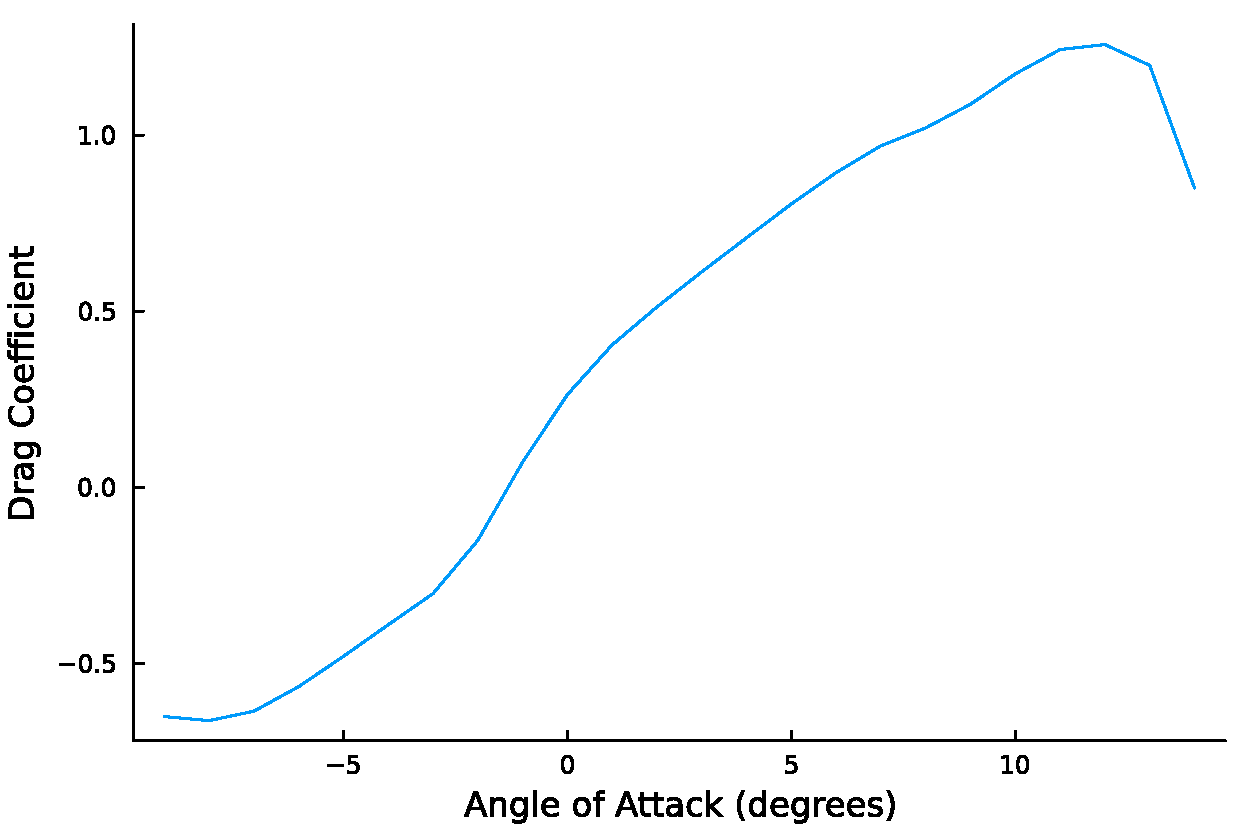
\includegraphics[width=\textwidth]{Updated Figures/Updated Figures 2/Lift New.pdf}
\caption{Lift of a NACA 2412 airfoil in flow with a Reynolds number of 100 thousand}
\label{fig:NACA 2412 Re=100000 Lift}
\end{minipage}
\begin{minipage}[b]{0.45\textwidth}
\centering
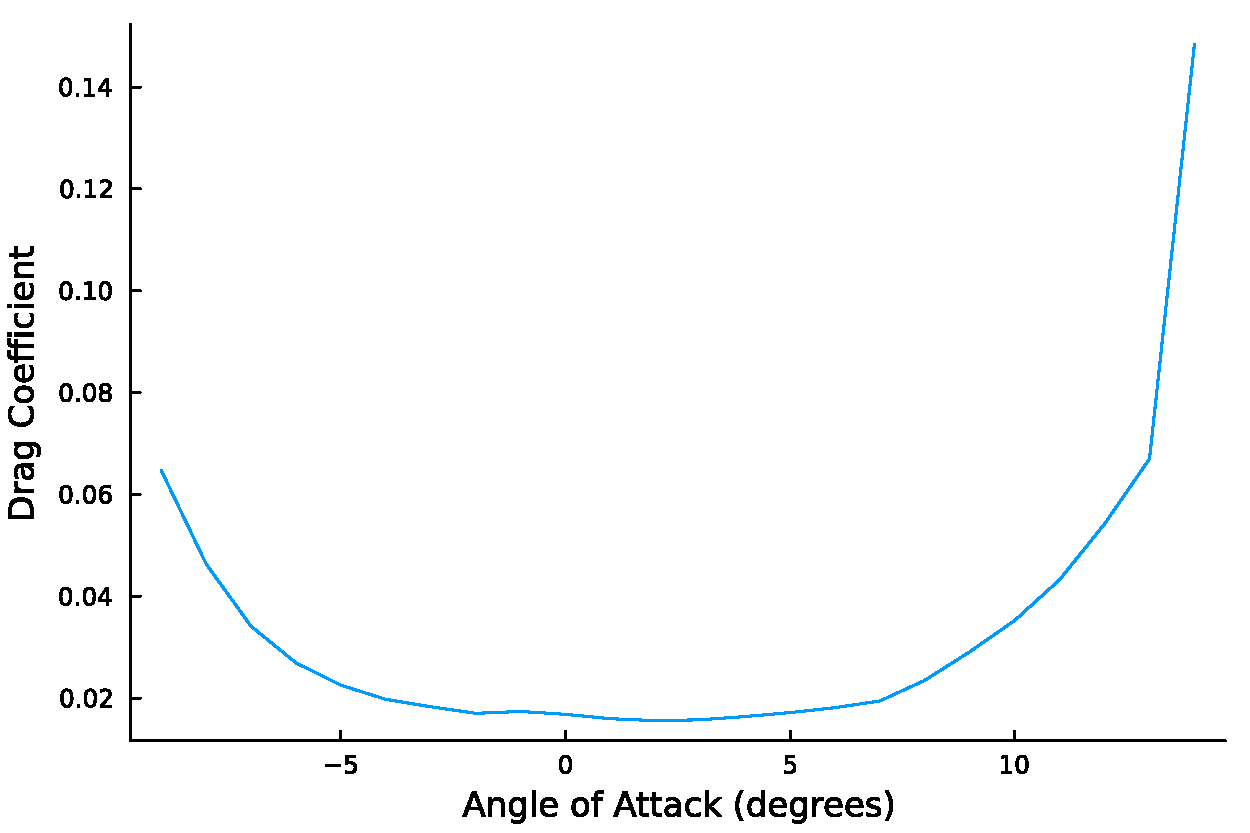
\includegraphics[width=\textwidth]{Updated Figures/Updated Figures 2/Drag New.pdf}
\caption{Drag of a NACA 2412 airfoil in flow with a Reynolds number of 100 thousand}
\label{fig:NACA 2412 Re=100000 Drag}
\end{minipage}
\end{figure}

\subsection{Drag Coefficient}
As shown in Figure \ref{fig:NACA 2412 Re=100000 Drag} the Drag coefficient increases with angle of attack, this change however is relatively gradual. However, once the Angle of Attack surpasses ten degrees it shoots up. This is likewise realted the stall angle of the airfoil, when the lift plummets the drag increases sharply. These forces together cause the plane to stall. To avoid insurmountable drag, the angle of attack must stay below the stall angle. Optimizing the angle of attack must consider both the total lift of the airfoil and the effect of drag and potential stalling.


\subsection{Moment Coefficient}
As shown in Figure \ref{fig:NACA 2412 Re=100000 Moment} the Moment coefficient stays relatively constant in the negative hundredths but fluctuates as lift and drag change. It increases as you move away from zero in either direction, with the minimum value near zero. Noticeably, as drag begins to sharply increase, the moment coefficient starts decreasing.

\begin{figure}[h]
\centering
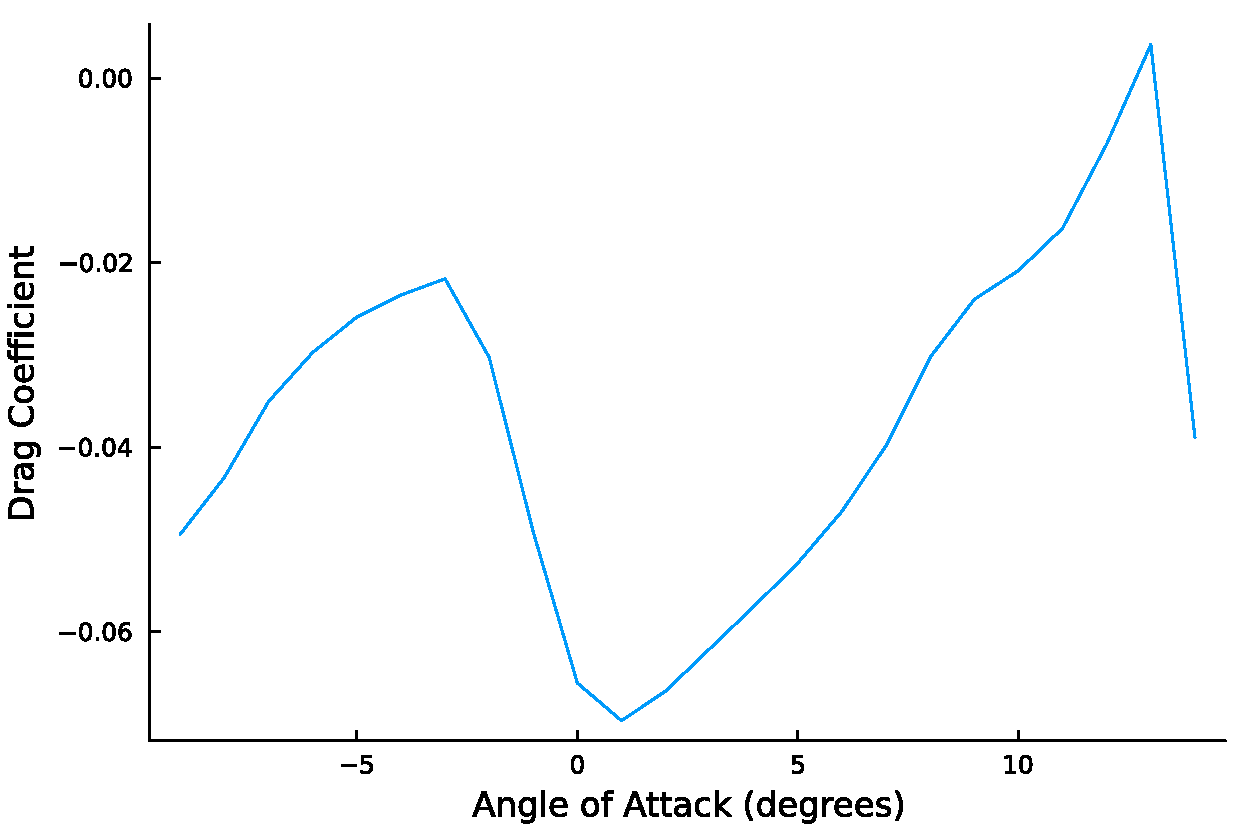
\includegraphics[width=.55\linewidth]{Updated Figures/Updated Figures 2/Moment New.pdf}
\caption{\label{fig:NACA 2412 Re=100000 Moment}Moment of a NACA 2412 Airfoil in Flow with a Reynolds Number of 100000}
\end{figure}

\section{Published Data Comparison}
Exploring how the panel method results from Xfoil compare  to published Xfoil data and experimental data for the same airfoil, we see a relatively close match. By comparing it to published data from Xfoil programs we can verify the functions are working as expected, while other comparisons help us evaluate the effectiveness of the panel method in general. In the experimental plots there are slight differences from the Xfoil data, but the overall trends are the same.

\subsection{Xfoil Comparisons}
Looking at Xfoil data generated by others for 6412 and 0012 NACA airfoils using a Reynolds number of 1 million, we can verify if our Xfoil code is providing realistic results \cite{aerotoolbox_lift_drag_moment}. Our moment coeficient calulcations match as shown in Figures  \ref{fig:Moment Comparison 6412}. However, Figure \ref{fig:Moment Comparison 0012} didn't match the Xfoil data from this source but covered approximately the same range of values. This indicated that these Xfoil functions use similar methodology to the one used by the authors of the article, yet there are potential differences in the particular NACA airfoil datasets used. This was confirmed by comparing the moment coefficient plot to a published plot from the source of the airfoil data points, showing an exact match (see Figure \ref{fig:Moment Comparison 0012}) \cite{naca0012h}. Comparing the drag and lift coefficients for each airfoil, we see exact matches although different ranges for the angle of attack were used, see Figures  \ref{fig:Lift Comparison} and \ref{fig:Drag Comparison}. Confirming that this panel method code functions as expected.

\begin{figure}[h]
    \centering
\begin{minipage}[b]{0.45\textwidth}
\centering
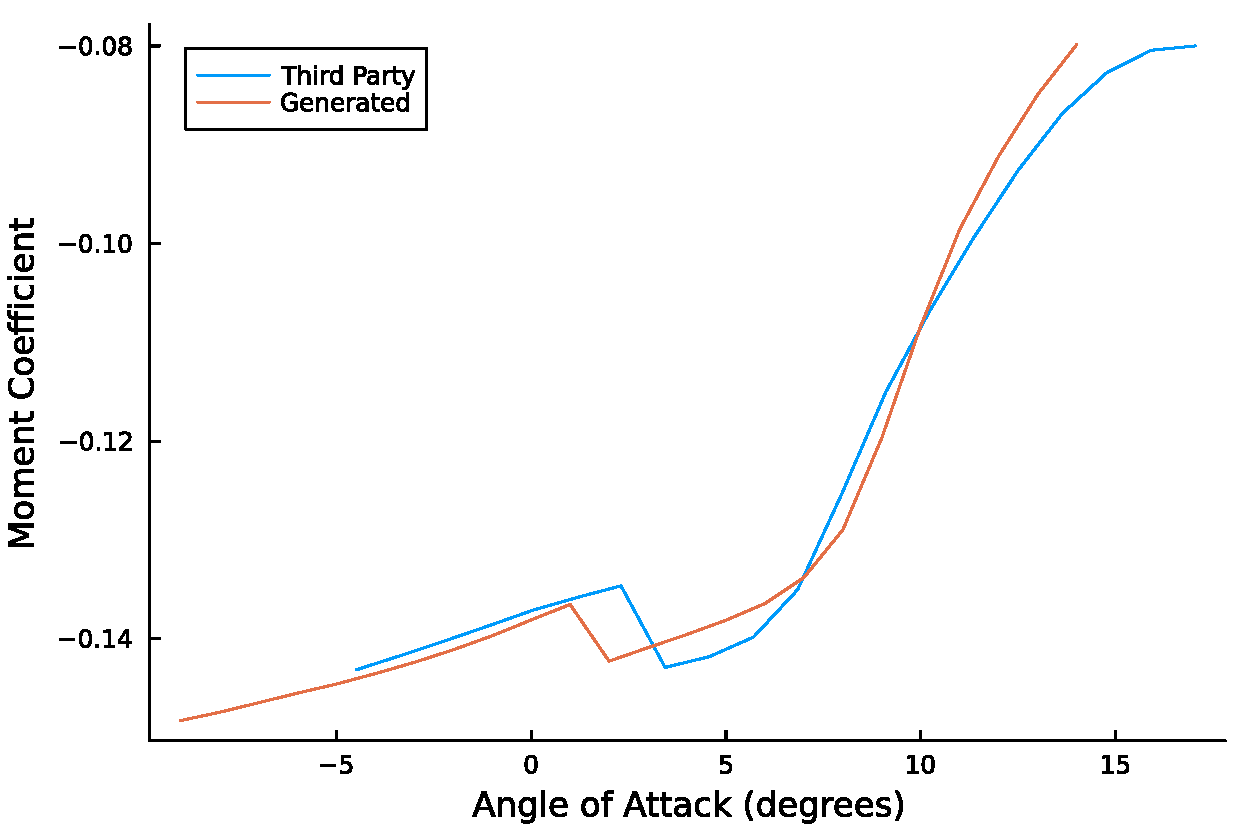
\includegraphics[width=\textwidth]{Updated Figures/Moment Comparison 6412.pdf}
\caption{\label{fig:Moment Comparison 6412}Moment coefficient Xfoil comparison, NACA 6412}
\end{minipage}
\begin{minipage}[b]{0.45\textwidth}
\centering
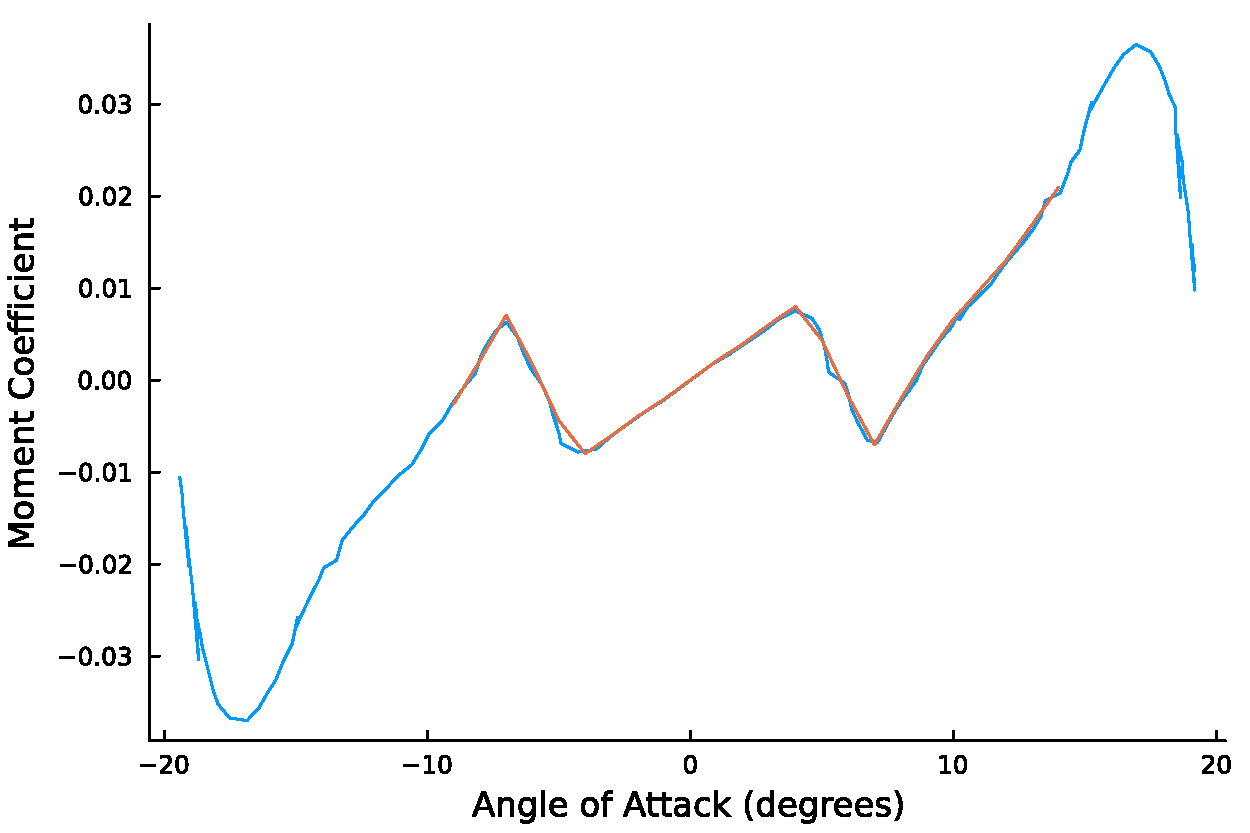
\includegraphics[width=
    \textwidth]{Updated Figures/Moment Comparison 0012.pdf}
    \caption{Moment coefficient Xfoil comparison, NACA 0012}
    \label{fig:Moment Comparison 0012}
\end{minipage}
\end{figure}
\begin{figure}[h]
    \centering
\begin{minipage}[b]{0.45\textwidth}
\centering
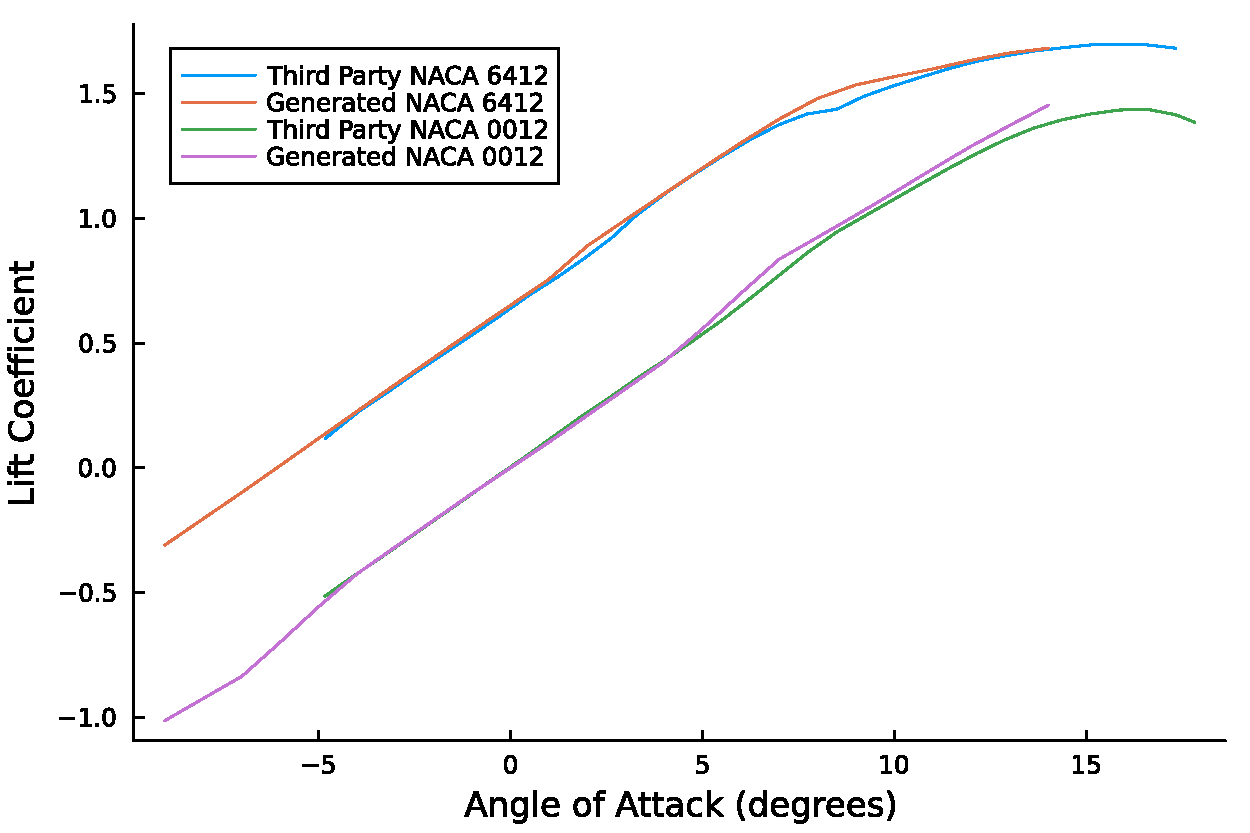
\includegraphics[width=\textwidth]{Updated Figures/Xfoil Lift.pdf}
\caption{\label{fig:Lift Comparison}Lift coefficient Xfoil comparison}
\end{minipage}
\begin{minipage}[b]{0.45\textwidth}
\centering
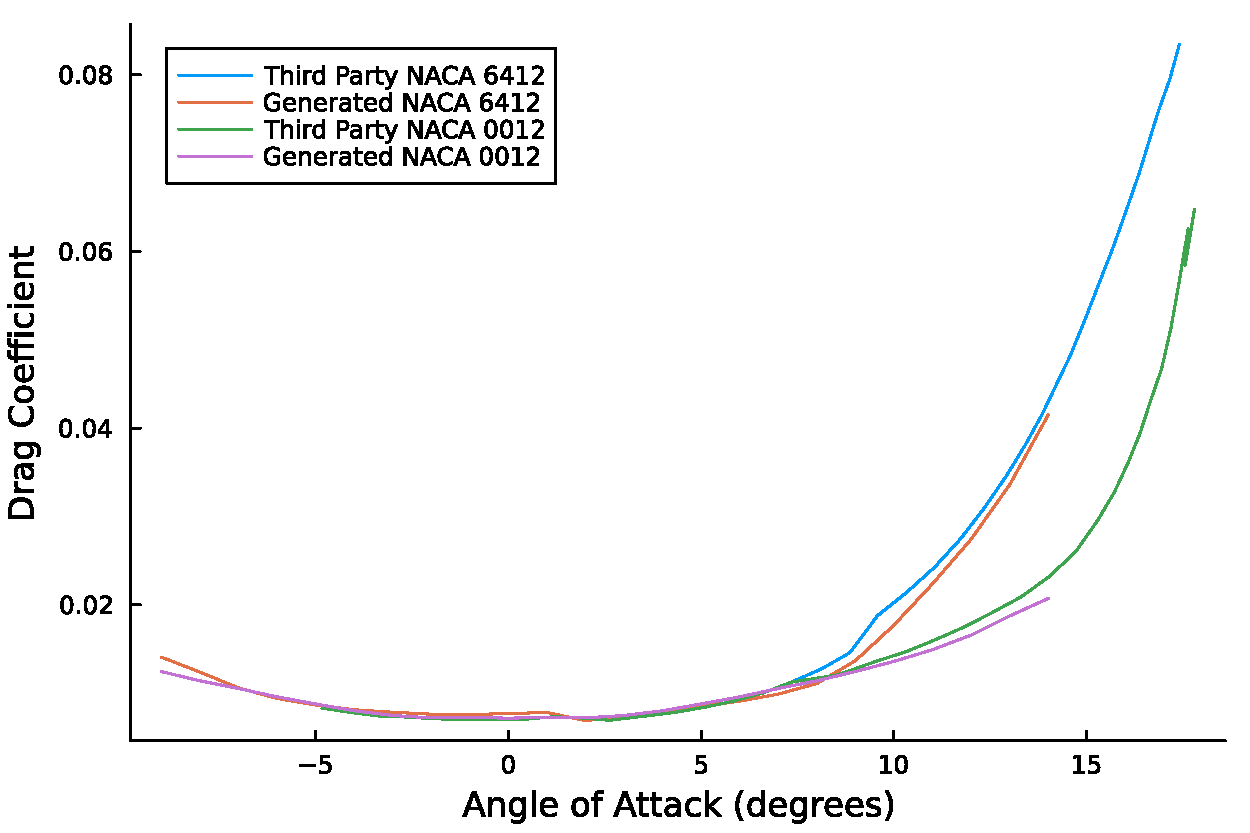
\includegraphics[width=\textwidth]{Updated Figures/Updated Figures 2/Xfoil Drag.pdf}
\caption{\label{fig:Drag Comparison}Drag coefficient Xfoil comparison}
\end{minipage}
\end{figure}

\subsection{Experimental Data Comparisons}

To compare with experimental data, I used a study conducted by NASA \cite{anderson1994simplified} in the 90's testing airfoils in a wind tunnel to verify the Xfoil data. Examining Figure \ref{fig:Exp 2412 Lift} we see that the experimental data is a near perfect match for our predicted lift coefficient. However, when comparing the drag coefficients, \ref{fig:Exp 2412 Drag}, we see that the generated Xfoil plot is a close match but not quite exact. This could be caused by the complexity and additional factors that play into drag in the real world which aren't accounted for in Xfoil. The values of the coefficients for these angle of attacks overall are really close, showing a good match between the experimental data and the Xfoil-generated plots.

\begin{figure}[h]
    \centering
\begin{minipage}[b]{0.45\textwidth}
\centering
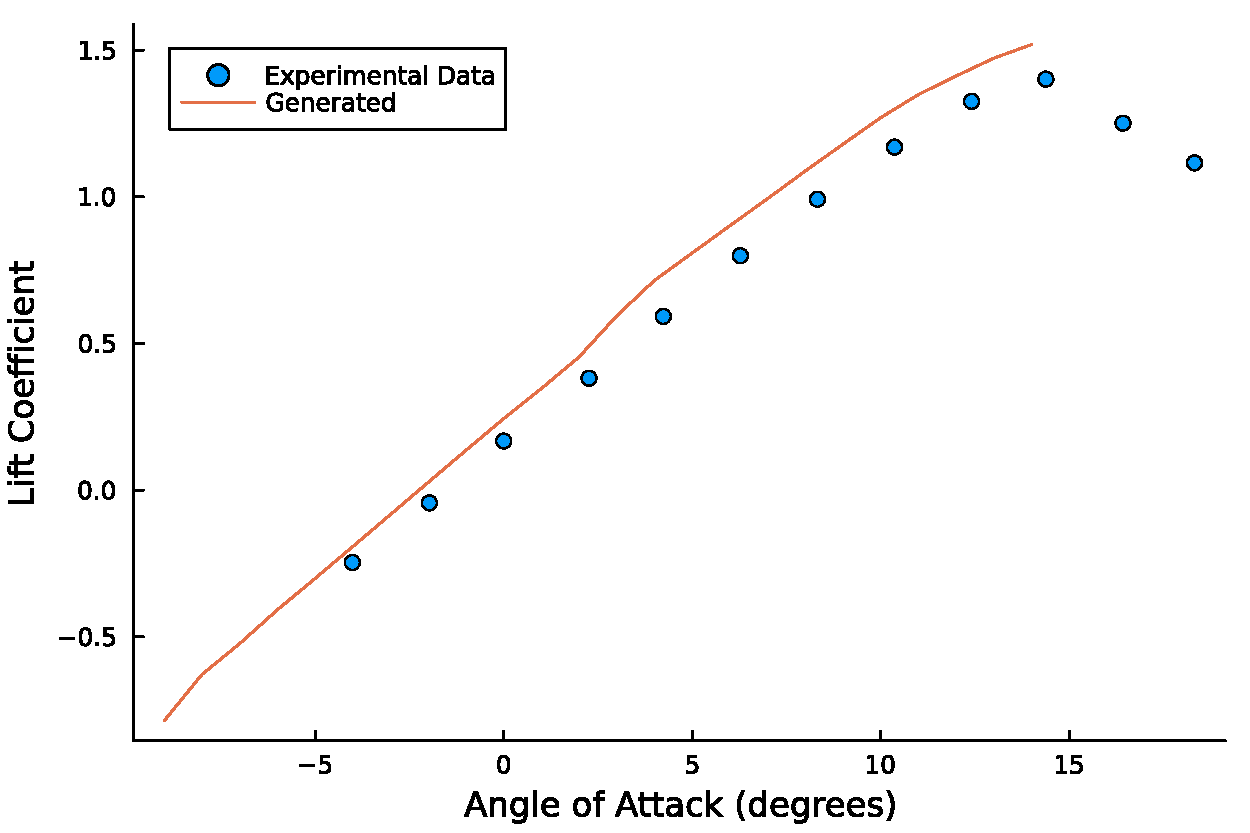
\includegraphics[width=\textwidth]{Updated Figures/Experimental Lift 2412.pdf}
\caption{\label{fig:Exp 2412 Lift}Lift coefficient comparison with experimental data, NACA 2412}
\end{minipage}
\begin{minipage}[b]{0.45\textwidth}
\centering
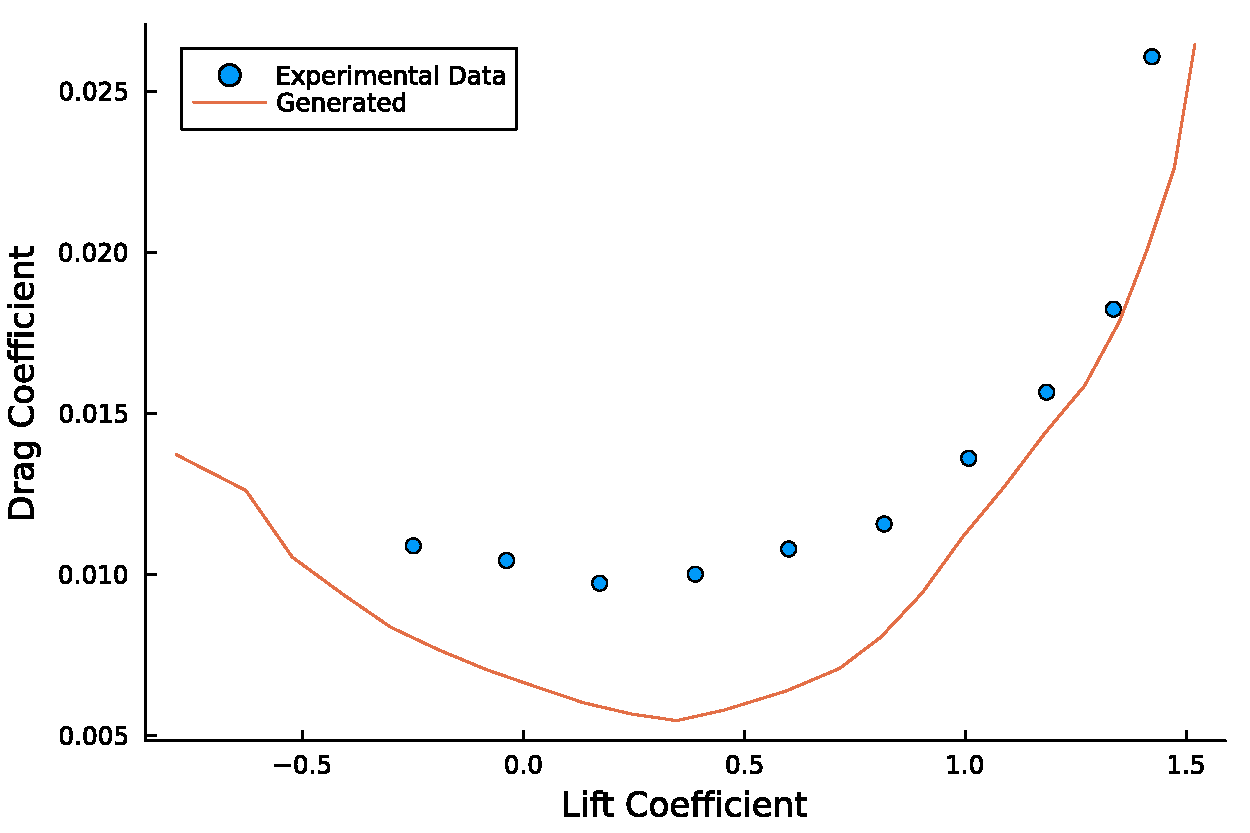
\includegraphics[width=\textwidth]{Updated Figures/Experimental Drag vs Lift 2412.pdf}
\caption{\label{fig:Exp 2412 Drag}Lift to drag ratio comparison with experimental data, NACA 2412}
\end{minipage}
\end{figure}

\begin{figure}[h]
    \centering
\begin{minipage}[b]{0.45\textwidth}
\centering
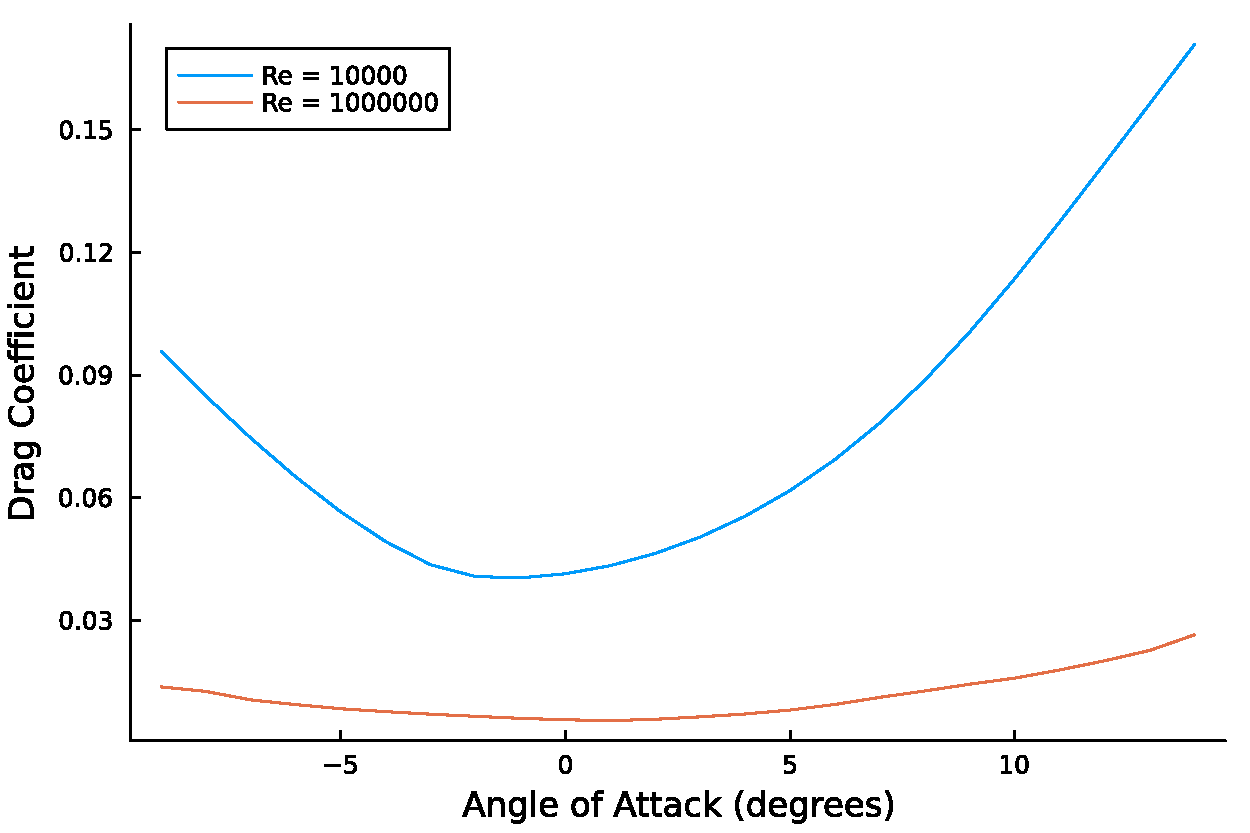
\includegraphics[width=\textwidth]{Updated Figures/Reynolds Drag 2412.pdf}
\caption{Effect of Reynolds number on drag}
\label{fig:Reynolds Drag}
\end{minipage}
\begin{minipage}[b]{0.45\textwidth}
\centering
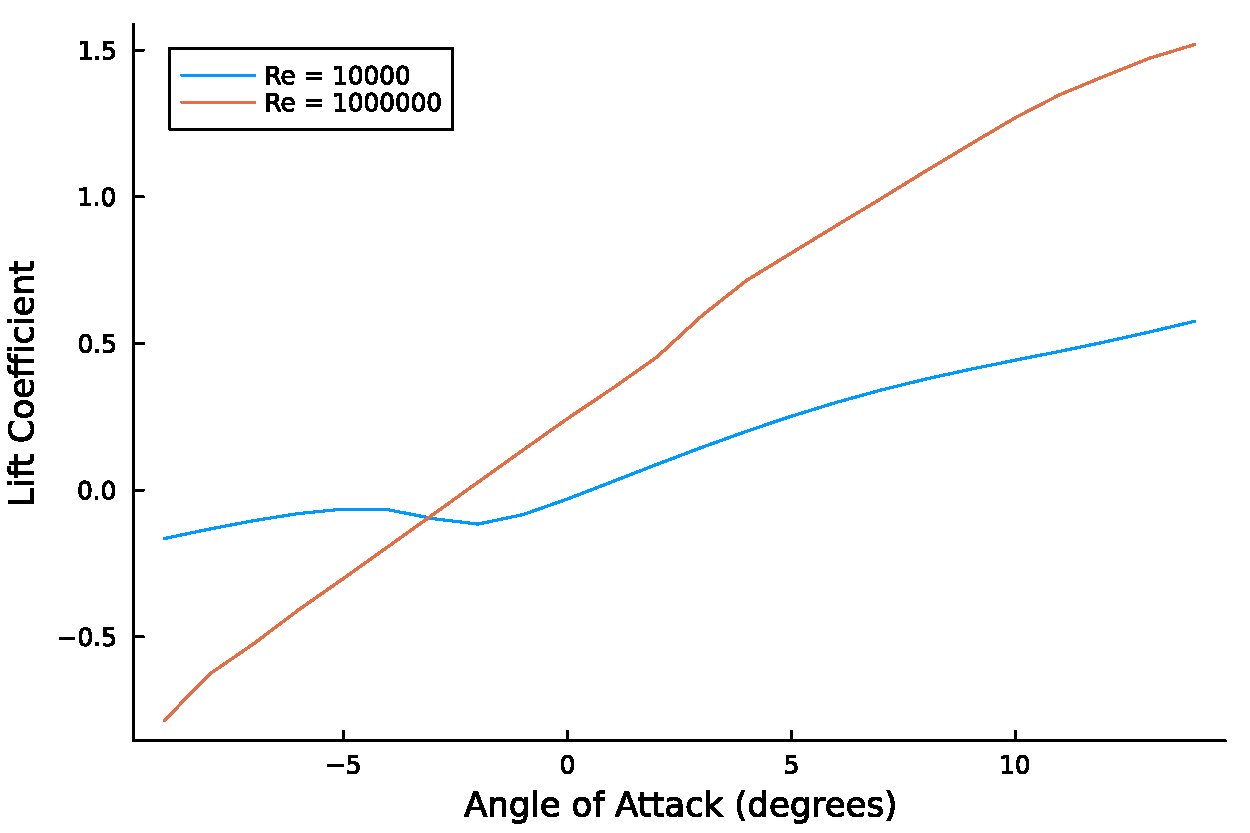
\includegraphics[width=\textwidth]{Updated Figures/Reynolds Lift 2412.pdf}
\caption{Effect of Reynolds Number on Lift}
\label{fig:Reynolds Lift}
\end{minipage}
\end{figure}

\begin{figure}
    \centering
    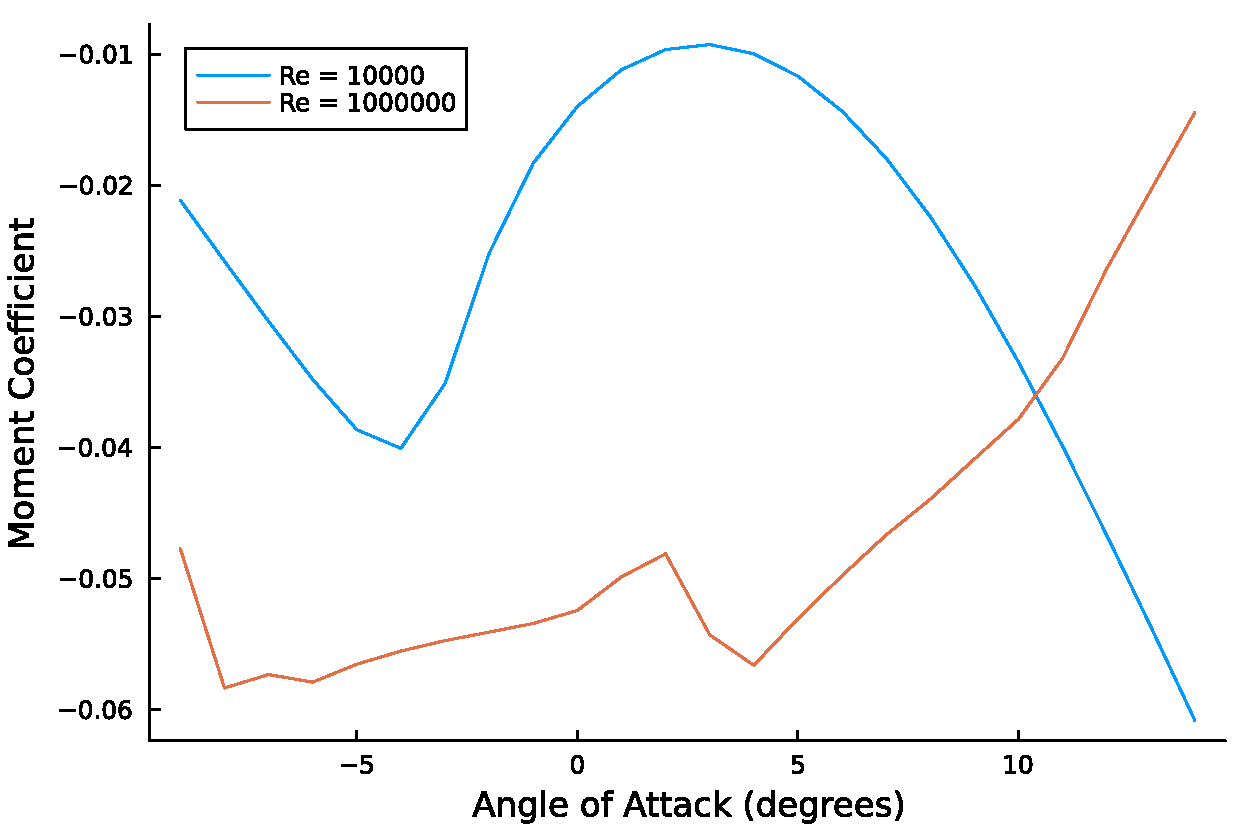
\includegraphics[width=0.5\linewidth]{Updated Figures/Reynolds Moment 2412.pdf}
    \caption{Effect of Reynolds Number on the Moment}
    \label{fig:Moment Reynolds}
\end{figure}

\subsection{Comparison Conclusion}
The Xfoil method aligns well with real data, CFD simulations, and other Xfoil programs. Overall, the panel method is accurate in estimating the lift, drag, and moment coefficients of a NACA airfoil for a given angle of attack and Reynolds number.

\section{Reynolds Number Effect}

The Reynolds number is a dimensionless value that represents the ratio of inertial to viscous forces. It characterizes the behavior of a fluid as it flows over a plate and determines if the flow is turbulent or laminar, affecting the lift, drag, and moment of the plane.

\subsection{Lift Coefficient}

As the Reynolds number increases the flow becomes more turbulent. Turbulent flow can follow sharper curves for longer, allowing the airfoil to handle more extreme angles of attack before stalling, as seen in Figure \ref{fig:Reynolds Lift}.

\subsection{Drag Coefficient}

At low angles of attack, the drag coefficient is similar, but it increases much quicker with higher Reynolds numbers due to more eddies and vortices. This increases boundary layer thickness which increases skin friction drag, and causes larger pressure differences increasing the pressure drag. This effect on the drag coefficient can be seen in Figure \ref{fig:Reynolds Drag}.

\subsection{Moment Coefficient}

As observed in Figure \ref{fig:Moment Reynolds}, the moment coefficient becomes more level and less responsive to changes in the angle of attack. This could be due to increased mixing, delayed separation of more turbulent flow, or perhaps the increased turbulence causes a more even pressure distribution.

\section{Effect of Airfoil Shape}
The shape of the airfoil significantly affects fluid flow impacting the lift, drag, and moment coefficients.
\subsection{Camber}
Camber, the curve or asymmetry of the wing, is one way to manipulate airfoil shape. It is the maximum distance between the chord line and a line equidistant between the upper and lower surfaces. For a symmetrical airfoil the camber is 0. 
\subsubsection{Lift to Drag Ratio}

Increased camber results in a positive shift in the lift to drag ratio, with greater periods of low drag and more rapid increases to higher drag coefficients. This can be seen in Figure \ref{fig:Camber Drag}.

\begin{figure}[h]
    \centering
\begin{minipage}[b]{0.45\textwidth}
\centering
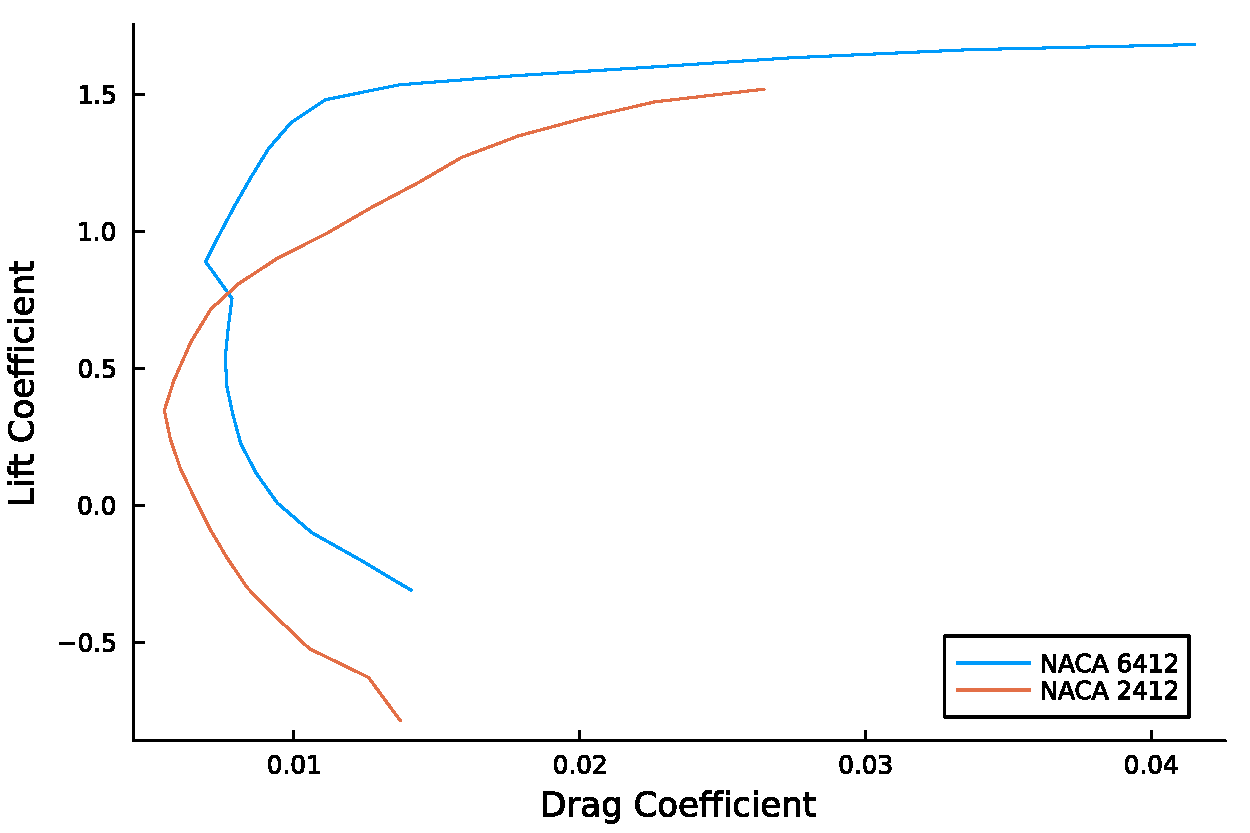
\includegraphics[width=\textwidth]{Updated Figures/Camber Lift Drag.pdf}
\caption{Effect of Camber on the lift to drag ratio}
\label{fig:Camber Drag}
\end{minipage}
\begin{minipage}[b]{0.45\textwidth}
\centering
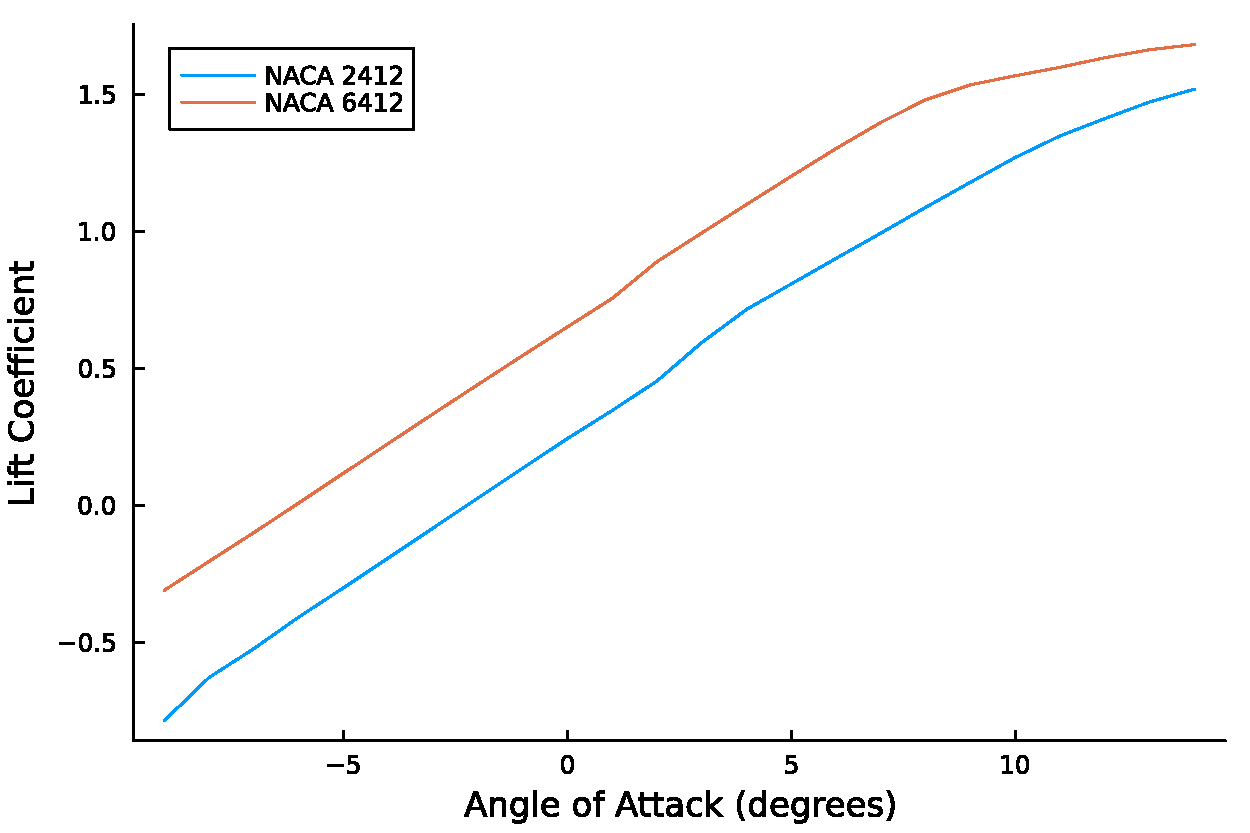
\includegraphics[width=\textwidth]{Updated Figures/Camber Lift.pdf}
\caption{Effect of Camber on Lift}
\label{fig:Camber Lift}
\end{minipage}
\end{figure}


\subsubsection{Lift Curve Slop}

The slope of the lift coefficient versus the angle of attack also experiences a positive shift with increased camber, as shown by Figure \ref{fig:Camber Drag}.


\subsection{Thickness}
Thickness, the maximum distance between the upper and lower surfaces of the airfoil perpendicular to the chord line, is another way we can manipulate the shape of the airfoil.

\subsubsection{Lift to Drag Ratio}
For thinner airfoils the lift coefficient plateaus or maxes out sooner when compared to the drag. This can be seen in Figure \ref{fig:Thickness Drag}.

\begin{figure}[h]
    \centering
\begin{minipage}[b]{0.45\textwidth}
\centering
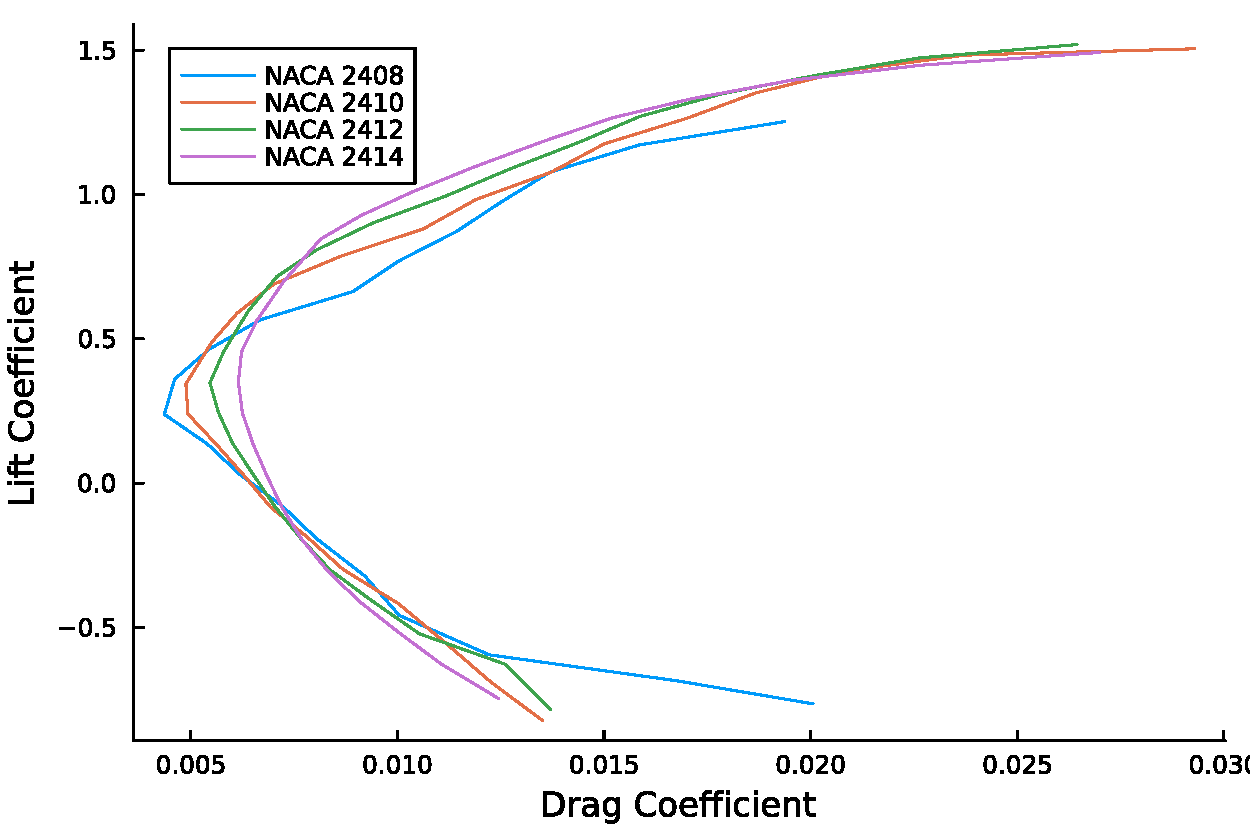
\includegraphics[width=\textwidth]{Updated Figures/Thickness Lift Drag.pdf}
\caption{Effect of thickness on the lift to drag ratio}
\label{fig:Thickness Drag}
\end{minipage}
\begin{minipage}[b]{0.45\textwidth}
\centering
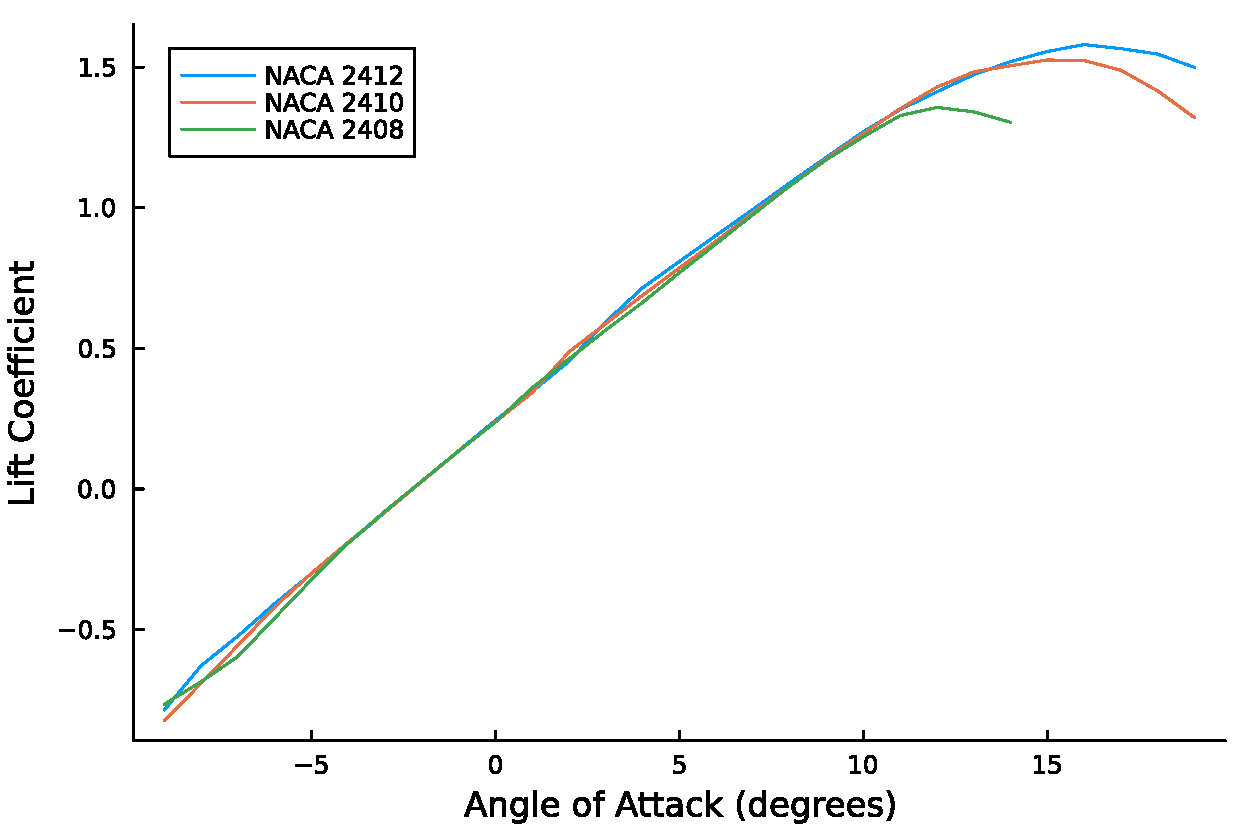
\includegraphics[width=\textwidth]{Updated Figures/Thickness Lift.pdf}
\caption{Effect of thickness on lift}
\label{fig:Thickness Lift}
\end{minipage}
\end{figure}

\subsubsection{Lift Curve Slope}
Thickness has little effect on the slope of the lift curve. However, it does seem to postpone the stall angle, shown by Figure \ref{fig:Camber Drag}.

\bibliographystyle{alpha}
\bibliography{sample}

\clearpage
\end{document}